\documentclass{beamer}
\usepackage{tikz}
\usetikzlibrary{positioning}

\usepackage{jobrad_colors}

\tikzset{
  history/.style={draw=green!50, fill=green!20},
  index/.style={draw=blue!50, fill=blue!20},
  working_directory/.style={draw=red!50, fill=red!20},
  branch/.style={draw=orange!50, fill=orange!20},
}

\title{Git Talk}
\author{Lukas Halbritter}
\date{2024}

\begin{document}

\frame{\titlepage}

\begin{frame}
  \begin{center}
    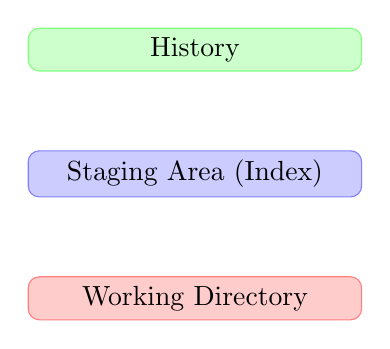
\begin{tikzpicture}
      [every node/.style={rounded corners, text width=4cm, align=center}]
      \node (history) [history] {History};
      \node (index) [index, below=of history] {Staging Area (Index)};
      \node (wd) [working_directory, below=of index] {Working Directory};
    \end{tikzpicture}
  \end{center}
\end{frame}

\begin{frame}
  \frametitle{JobRad color scheme sample}
  \begin{center}
    \begin{tikzpicture}
      [every node/.style={rounded corners, minimum width=3cm, align=center, minimum height=8mm}]
      \node (anthrazit1) [fill=anthrazit1] {Anthrazit 1};
      \node (anthrazit2) [fill=anthrazit2, below=4mm of anthrazit1] {Anthrazit 2};
      \node (anthrazit3) [fill=anthrazit3, below=4mm of anthrazit2] {Anthrazit 3};
      \node (anthrazit4) [fill=anthrazit4, below=4mm of anthrazit3] {Anthrazit 4};
      \node (anthrazit) [fill=anthrazit, below=4mm of anthrazit4] {Anthrazit};
      \node (anthrazit5) [fill=anthrazit5, below=4mm of anthrazit] {Anthrazit 5};
      \node (pink) [fill=pink, right=4mm of anthrazit1] {Pink};
      \node (pink1) [fill=pink1, below=4mm of pink] {Pink 1};
      \node (pink2) [fill=pink2, below=4mm of pink1] {Pink 2};
      \node (pink3) [fill=pink3, below=4mm of pink2] {Pink 3};
      \node (pink4) [fill=pink4, below=4mm of pink3] {Pink 4};
      \node (pink5) [fill=pink5, below=4mm of pink4] {Pink 5};
      \node (mg1) [fill=maigruen1, right=4mm of pink] {Maigrün 1};
      \node (mg) [fill=maigruen, below=4mm of mg1] {Maigrün};
      \node (mg2) [fill=maigruen2, below=4mm of mg] {Maigrün 2};
      \node (mg3) [fill=maigruen3, below=4mm of mg2] {Maigrün 3};
      \node (mg4) [fill=maigruen4, below=4mm of mg3] {Maigrün 4};
      \node (mg5) [fill=maigruen5, below=4mm of mg4] {Maigrün 5};
    \end{tikzpicture}
  \end{center}
\end{frame}
\end{document}
